\documentclass[12pt]{article}
\usepackage{graphicx}
\usepackage[utf8]{inputenc}
\usepackage[ngerman]{babel}
\usepackage[T1]{fontenc} 
\usepackage{wrapfig}




\begin{document}


\begin{titlepage}
\newcommand{\HRule}{\rule{\linewidth}{0.5mm}}
\center

\textsc{\LARGE Hochschule Kempten}\\[0.5cm]
\textsc{\large Fakultät Informatik}\\[0.5cm]
\textsc{\large Masterstudiengang Angewandte Informatik}\\[1.5cm]

\HRule \\[0.4cm]
{\huge \bfseries Verhaltensausbreitung}\\[0.2cm]
\HRule \\[1.0cm]

\textsc{\LARGE Seminararbeit}\\[0.5cm]
\textsc{\large im Seminar}\\[0.5cm]
\textsc{\LARGE Informationssuche, Soziale Netzwerke, Moderne Algorithmen}\\[1.5cm]



\begin{minipage}{0.4\textwidth}
\begin{flushleft}\large
\emph{Autor:}\\
Fabian Thomas \textsc{Schafroth}
\end{flushleft}
\end{minipage}
~
\begin{minipage}{0.4\textwidth}
\begin{flushright}\large
\emph{Betreuer:}\\
Prof. Dr. Jochen \textsc{Staudacher}
\end{flushright}
\end{minipage}\\[4cm]
{\large \today}\\[3cm]

%includegraphics{logo}\\[1.0cm]

\vfill
\end{titlepage}
\newpage
	\pagenumbering{roman}
	\tableofcontents
\newpage
\pagenumbering{arabic}

\section{Einführung}
Das Aufkommen von neuen Verhaltensweisen und deren Verbreitung in sozialen Netzen, sind Phänomene, die sowohl in tierischen als auch in menschlichen Gemeinschaften beobachtet werden können und von wissenschaftlichem Interesse sind. Ein Individuum innerhalb einer Gemeinschaft ist unter normalen Umständen stets bestrebt, sich den Normen und Verhaltensweisen der Mehrheit anzupassen. Dieses Verhalten lässt sich damit begründen, dass homogene Gemeinschaften besonders gut funktionieren. Solche Gemeinschaften unterscheiden sich von heterogenen besonders darin, dass sie sich aus Individuen zusammen setzten, welche große Übereinstimmungen in ihrer Art, Sprache und Verhalten aufweisen[QUOTERoger]. Diese homogenen Individuen halten einen engen Kontakt zueinander, tauschen sich oft aus und schätzen die jeweilige Meinung der anderen. Zudem werden vertraute Personen im nahen sozialen Umfeld bereitwilliger als Vorbilder akzeptiert als fremde Menschen.\\\\
Die auf diese Situation aufbauende Theorie der Verhaltensausbreitung geht als Grundlage davon aus, dass ein Individuum stets sein nahes soziales Umfeld betrachtet und Veränderungen darin wahrnimmt sowie sie gegebenenfalls auf ihren Nutzen hin analysiert. Sollte sich in diesem Umfeld eine Änderung in der Verhaltensweise vollzogen haben, wird das Individuum früher oder später nachziehen, sofern es einen tatsächlichen (oder auch nur gefühlten) Vorteil darin sieht. Was mit der Einführung eines neuen Verhaltens hier konkret gemeint ist kann vielfältig sein. Die Verwendung einer neuen Technologie zum Ackerbau, ein neuer Kleidungsstil oder ein schnellerer Web Browser.\\\\
Der Beginn einer jeden Verhaltensausbreitung beginnt folglich damit, dass ein oder mehrere Individuen aus eigenen Stücken, ohne Einfluss durch ihr nahes soziales Umfeld, ein neues Verhalten annehmen. Von diesen Pionieren ausgehend kann sich dieses Verhalten innerhalb der Gemeinschaft verbreiten durch die zuvor bereits genannten, engen Beziehungen. Dieser Vorgang wird als Kaskade bezeichnet, eine Ausbreitung ähnlich einer Kettenreaktion deren endgültiges Ziel (Equilibrium) dann erreicht ist wenn alle Individuen einer Gemeinschaft das durch die Kaskade verbreitete, neue Verhalten angenommen haben.
Kaskaden lassen sich bezüglich mehrerer Faktoren auf ihren Erfolg hin analysieren.
\begin{enumerate}
\item Wie schnell verbreitet sich eine Kaskade
\item Was für Bedingungen sind für die Verbreitung von Bedeutung
\item Gibt es innerhalb von sozialen Netzwerken natürliche Hindernisse
\item Gelingt es einer Kaskade ein Equilibrium herbeizuführen
\end{enumerate}
Besonders interessant sind Kaskaden und ihre Effekte natürlich für das moderne Marketing da man möglichst akkurate Modelle erstellen möchte um neue Produkte am Markt bestmöglich zu verbreiten und künstlich Trends zu setzen. Eine gänzlich neue Dimension haben in diesem Bereich die Internetmedien und darin entstandenen online sozialen Netzwerke geschaffen.\\\\



\section{Verhaltensausbreitung}
Nach Rogers lässt sich die Verhaltensausbreitung auf vier übergeordnete Aspekte konzentrieren. Die Innovation welche neu in  einem sozialen Netzwerk aufgekommen ist. Die Kommunikationskanäle welche innerhalb dieses Netzwerkes bestehen und damit auch das soziale Gefüge definieren. Die Zeit welche in mehreren Blickwinkeln maßgeblich den Erfolg einer Verhaltensausbreitung definiert.
\subsection{Innovation}
Als Innovation wird gemeinhin ein neues Verhalten bezeichnet, welches von den Mitgliedern eines sozialen Netzwerkes entweder adaptiert oder abgelehnt werden kann. Für welche der beiden Wahlmöglichkeiten sich die Individuen entscheiden, hängt im Rahmen der Betrachtung von Kaskaden maßgeblich davon ab, wie viele benachbarte Kontakte sich bereits für das neue Verhalten entschlossen haben. Entgegen diesem rein mathematischen Ansatz beschäftigt sich dieser Abschnitt detaillierter mit den soziologischen Faktoren warum eine Innovation Erfolg hat oder nicht.\\\\
Rodgers definierte fünf Attribute welche mit unterschiedlicher Gewichtung dazu beitragen ob die Kaskade einer Innovation sich über ein gesamtes Netzwerk verbreiten kann.
\begin{enumerate}
\item \textbf{Relativer Vorteil}\\ Als relativer Vorteil einer Innovation lässt sich das Gefühl umschreiben, nach welchem die Individuen eines sozialen Netzwerkes einen Vorteil für sich darin sehen ein neues Verhalten zu adaptieren. Es wird dabei großen Wert auf die Tatsache gelegt, dass es nicht nötig ist, dass die Innovation einen tatsächlich quantitativ oder empirisch erfassbaren Vorteil bringt.
\item \textbf{Kompatibilität}\\ Die Kompatibilität einer Innovation bestimmt wie gut die Innovation mit dem vorherrschenden Normen und Wertesystem einer Gemeinschaft im Einklang ist. Je gegenläufiger diese beiden Konzepte zu einer möglichen Innovation sind, desto schwerer wird sie es haben sich innerhalb der homogenen Gemeinschaft durchzusetzen.
\item \textbf{Komplexität}\\ Die Komplexität einer Innovation beschreibt wie schwierig es für ein Individuum ist sie zu adaptieren. Hieraus lässt sich leicht der Schluss ziehen, dass natürlich je einfacher zu verstehen eine Innovation ist, desto schneller werden viele Menschen die adaptieren. Smartphones, zum Beispiel, haben sich nicht am Markt durchgesetzt, weil sie fürchterlich kompliziert zu bedienen sind.
\item \textbf{Erprobbarkeit} \\ Am Klassischen Beispiel der Verbreitung von Hybriden Mais-Samen unter Farmern in Iowa lässt sich erkennen, welche Bedeutung die Erprobbarkeit einer Innovation hat. Kaum einer der Farmer hätte sich für die neuen Samen entschlossen, wenn er von einem Tag auf den anderen mit seinem kompletten Anbaugebiet auf die neuen Samen hätte wechseln müssen. Stattdessen testeten die meisten Bauern die neuen Samen erst auf einem kleinen Teil ihres Ackers und als dieser gute Erträge abwarf wechselten sie dann komplett.
\item \textbf{Beobachtbarkeit} \\ Individuen tauschen sich innerhalb eines engen sozialen Netzwerkes nicht nur verbal aus, sondern beobachten sich auch gegenseitig. Daher ist es für eine Innovation besonders nützlich, wenn ihr (vermeintlich oder tatsächlicher) Vorteil gut sichtbar für jeden ist.
\end{enumerate}
\subsection{Das soziale Netzwerk}
Neben den im vorherigen Abschnitt beschrieben Qualitäten, welche eine Innovation besitzt um ihre Verbreitung voran zu treiben, ist auch die Struktur des sozialen Netzwerkes von großer Bedeutung. Wie im Kapitel zur Modellierung von Netzwerken dargelegt wird gibt es bestimmte Strukturen innerhalb der Kommunikationskanäle (Bekanntschaften) eines Netzwerkes welche sich entweder förderlich aber auch hemmend auf die Verbreitung einer Innovation hin auswirken können.
\begin{figure}
  \begin{center}
    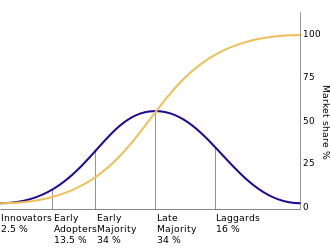
\includegraphics[width=0.80\textwidth]{pic_diffusion.png}
  \end{center}
  \caption{Zusammenspiel zwischen Personentypen und Innovation}
  WIKIPEDIA article DIFFUSION
  \label{pic_diffusion}
\end{figure}

\subsubsection{Personen}
Die für die Verhaltensausbreitung relevanten Personen eines sozialen Gefüges lassen sich in fünf Kategorien unterteilen, welche durch die Zeit als Dimension definiert werden. Genauer die Zeit zu welcher sie sich entschließen eine Innovation anzunehmen.
\begin{enumerate}
\item \textbf{Innovatoren} Innovatoren sind die ersten Personen innerhalb eines sozialen Netzwerkes welches sich einer neuen Innovation annehmen und sie adaptieren. Diese Personen haben meist eine herausragende soziale oder intellektuelle Stellung innerhalb einer Gemeinschaft. Ihre Beziehungen reichen über sogenannte Weak Ties (beschrieben kap bla) weit über das unmittelbare soziale Netz hinaus. Somit erfahren sie früher als andere von neuen Innovationen.
\item \textbf{Frühzeitiger Anwender} Diese Personengruppe hat meist einen direkten Kontakt zu den Innovatoren und ist somit prädestiniert, ein Verhalten sehr Früh in der Zeitlinie einer Verhaltensausbreitung zu adaptieren. Der größte Unterschied zwischen den frühzeitigen Anwendern und den Innovatoren ist, dass sie im Gegensatz zu letzteren bereits durch Observation innerhalb ihres sozialen Umfeldes sich zum Verhaltenswechsel entschlossen haben.
\item \textbf{Frühe und späte Mehrheit} Diese beiden Klassen sind von allen Personen prozentual die größte Gruppe. Die Unterscheidung zwischen früher und später Mehrheit ist rein zeitlicher Natur da zwischen den Mitgliedern dieser Gruppe untereinander kein bemerkenswerter sozialer oder gesellschaftlicher Unterschied besteht.
\item \textbf{Nachzügler} Nachzügler stehen am Ende der Kette und adaptieren ein neues Verhalten erst dann wenn fast schon das gesamte soziale Netz hin zu dieser Innovation gewechselt ist. Sie besitzen innerhalb einer Gesellschaft häufig einen niederen Stand oder verfügen über wenige soziale Verknüpfungen sowie eine geringe Innovationsbereitschaft.
\end{enumerate}
\subsubsection{Kanäle der Verhaltensausbreitung}
Damit ein Individuum überhaupt auf die Idee kommt sein momentanes Verhalten durch ein neues zu ersetzen, muss als grundsätzliche Annahme gegeben sein, dass das Individuum von diesem neuen Verhalten über einen seiner Sinne Kenntnis genommen hat. Entweder er hat die Vorzüge des neuen Verhaltens selbst gesehen oder von einem Freund oder aus den Nachrichten davon gehört. Die Kanäle über welche sich die Information über eine neue Innovation verbreiten sind so vielfältig das es den Rahmen dieser Arbeit sprengen würde sie in großem Detail zu betrachten. Allerdings biete sich die nähere Analyse von zwei Obergruppen an, über welche sich Informationen in sozialen Gemeinschaften verbreiten.
[Quelle Paper von Granovetter als Hauptquelle für diesen Abschnitt]
\paragraph{Strong Ties}
Unter Strong Ties (Starke Verknüpfungen) wird in einer Gemeinschaft die unmittelbare soziale Umgebung eines Individuums verstanden. Diese besteht aus sehr nahen Verwandten, Bekannten und Freunden. Zu ihnen hat das Individuum eine sehr enge Verknüpfung, es schätzt ihre Meinung und meistens teilt es auch Verhaltensweisen sowie Interessen. Dies ergibt sich aus dem natürlichen Bestreben eines Individuums, sich mit Personen zu umgeben die ihm ähnlich sind. Strong Ties spielen bei der Verhaltensausbreitung die maßgebliche Rolle, da hauptsächlich über sie die Verbreitung einer Innovation stattfindet, welche im Endeffekt zu einer Adaption führt. Es hat deutlich mehr Gewicht für ein Individuum, wenn einer seiner besten Freunde ein neues Verhalten adaptiert, als wenn es ein flüchtiger Bekannter tut. Während die Strong Ties folglich sehr förderlich für die Verhaltensausbreitung sind, so haben sie einen sehr großen Nachteil was die pure Informationsverbreitung betrifft. Gerade weil die soziale Struktur innerhalb eines Netzwerks aus Strong Ties stark verknüpft ist gibt es darin wenig neue Information. Die Informationen welche ein Individuum von einem besten Freund oder nahem Verwandten bekommen kann hat es wahrscheinlich schon erfahren.
\paragraph{Weak Ties}
Diese im vorherigen Abschnitt angesprochene flüchtige Bekanntschaft wäre nach der Definition von Verhaltensausbreitung in sozialen Netzen ein sogenannter Weak Tie (schwache Verknüpfung). Weak Ties finden sich in Gemeinschaften oftmals als Brücken zwischen einzelnen sozialen Gruppen. Ein Individuum \textbf{P} aus Gruppe \textbf{A} kennt ein Individuum \textbf{Q} aus Gruppe \textbf{B}. Sonst kennt \textbf{P} niemanden aus Gruppe \textbf{B} und \textbf{Q} kennt niemanden sonst aus Gruppe \textbf{A}. Diese Verteilung der Bekanntschaften ist exemplarisch für einen Weak Tie. Zum einen, da sie konträr zu der Definition eines Strong Tie fährt. Andererseits da sich über sie nur sehr selten eine Verhaltensausbreitung vollziehen wird, was daran liegt, dass Weak Ties oftmals sogenannte Cluster innerhalb eines Netzwerkes verbinden. Die Bedeutung von Cluster für die Verhaltensausbreitung wird in einem späterern Kapitel verdeutlicht. Warum diese Verbindungen trotzdem indirekt für die Verhaltensausbreitung wichtig sind legte Granovetter[QUOTE] dar. Beispielsweise besitzen Innovatoren oft Weak Ties die ihnen Verbindungen in andere soziale Netzwerke ermöglichen. Über diese Verbindungen erfahren sie dann vielleicht von Innovationen welche ihr eigenes Umfeld noch nicht erreicht haben.
\subsection{Zeit als Faktor}
Die Zeit als Faktor findet sich in drei Bereichen einer Verhaltensausbreitung wieder.
\begin{enumerate}
\item Der Entscheidungsfindungsprozess durchläuft entlang der Zeitachse mehrere Stufen in welchen sich das Individuum vom erstmaligen Hören einer Innovation bis hin zu dessen Adaption vorarbeitet. Wie schnell dies geschieht ist abhängig von den sozialen Strukturen und der Einstellung der Person selbst.
\item In welches Spektrum der Personen [LINK] ein Individuum zuzuordnen ist hängt maßgeblich davon ab, wann es sich dazu entscheidet eine Innovation anzunehmen. Während Innovatoren den Startschuss setzen entschließen Nachzügler sich erst sehr spät im Prozess der Verhaltensausbreitung eine Adaption in Betracht zu ziehen.
\item Der dritte Faktor ist definiert als die Rate der Adaption welche sich durch die Anzahl der Individuen berechnet, welche in einem gegebenen Zeitintervall ein neues Verhalten angenommen haben.
\end{enumerate}

\subsection{Historische Beispiele}
Die Standardbeispiele oder vielleicht hier auch bezug zu einem aktuelleren Beispiel falls sich etwas finden lässt, das wäre sicherlich gut damit hier nicht wieder über Korn oder APothekenprodukte geredet wird wie es schon in all den anderen Papers zu dem Thema der Fall ist. Dann natürlich auch den Titel dementsprechend anpassen. Wenn ich ein Aktuelleres Beispiel nehmen kann ich dann auch besser Bezug nehmen zu den momentanen Umständen und die unglaubliche SChlagkraft welche das Thema durch Soziale Netzwerke und Twitter und CO erhalten hat.

\section{Modellierung eines soziale Netzwerks}
Wie im vorangegangenen Kapitel dargelegt wurde sind die Hauptaspekte bei der Betrachtung eines sozialen Netzwerkes die in ihm befindlichen Individuen sowie deren Beziehungen untereinander. Dieser Umstand lässt sich mithilfe von gängigen Mustern und Darstellungsformen aus der Graphentheorie besser und formal strukturierter darstellen.\\\\

\begin{figure}
  \begin{center}
    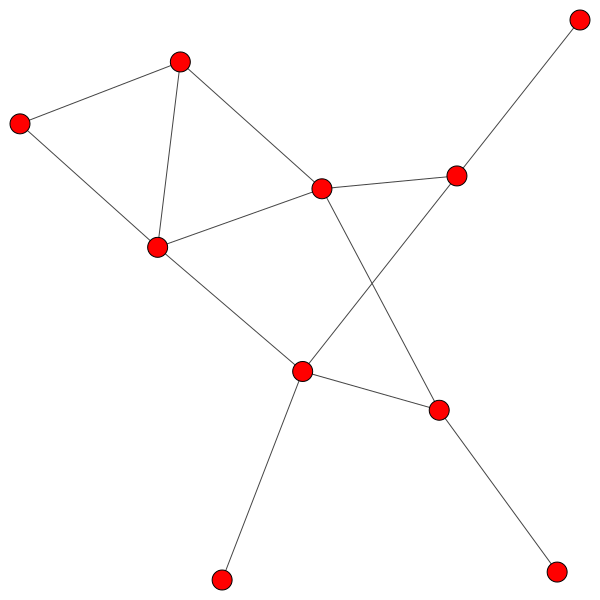
\includegraphics[width=0.60\textwidth]{pic_simpleGraph.png}
  \end{center}
  \caption{Ein einfacher bidirektionaler Graph}
\end{figure}


Die Modellierung eines sozialen Netzwerks baut auf dem Prinzip eines ungerichteten Graphen auf bei dem die Knoten Individuen sind und die Kanten Bekanntschaften welche die Individuen miteinander teilen. Das ein solcher Graph ungerichtet ist wird formal darum angenommen, da eine Kommunikation zwischen zwei Individuen für die betrachteten Netzwerke als bidirektional angesehen wird. Zudem wird, um ein möglichst realistisches Abbild zu schaffen, davon ausgegangen, dass die Graphen sehr sparse sind [Paper von Watts].
\subsection{Formale Definition und Bedingungen}
Die Bedingungen und formalen Definitionen welche MORRIS in seinem Paper für einen Graphen aufstellt welcher zur Untersuchung von Verhaltensausbreitung erforscht werden soll.
\subsection{Besondere Netzwerkkonstrukte}
Zwar kann man für die Untersuchung von Verhaltensausbreitung in sozialen Netzwerken auch zufällig generierte Graphen verwenden, sofern sie den formalen Anforderungen genügen. Doch sind soziale Strukturen, welche mithilfe solcher Graphen abstrahiert werden sollen, mitnichten zufällig sondern entsprechen oft vordefinierten Mustern.\\ Daher ist es von Interesse besonders häufig auftretende oder die Ausbreitung stark beeinflussende Konstrukte gesondert zu betrachten.
\subsubsection{Weak Tie - Strong Tie}
Wie im Kapitel [KAP] bereits dargelegt gibt es mit Strong- und Weak Ties zwei grobe Gruppen in die sich sämtliche Verbindungen innerhalb eines Netzwerkes klassifizieren lassen. Abbildung [ABB] zeigt ein typisches, einfaches Beispiel für einen Graph mit klar erkennbaren Strong- und Weak Ties (starke Kanten sind Rot markiert und schwache Blaue).\\
Beispiel für ein Netzwerk in dem die Weak Ties und Strong Ties separat hervorgehoben sind besonders natürlich im Bezug auf die Erklärung welche zuvor zu diesen Verbindungen abgegeben wurde.

\begin{figure}
  \begin{center}
    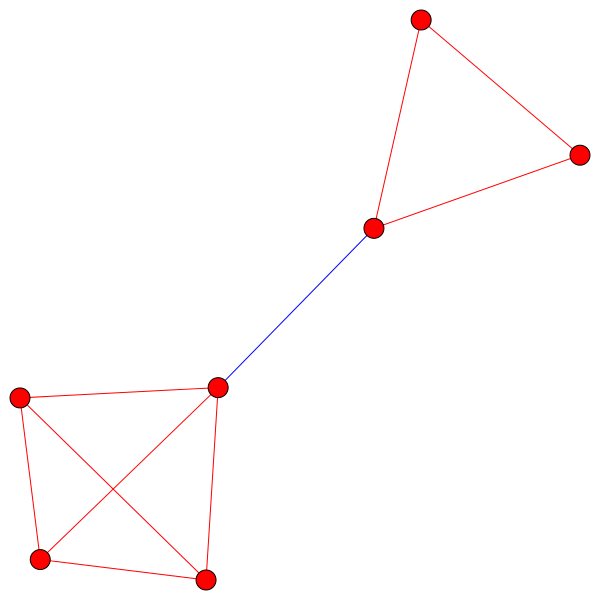
\includegraphics[width=0.60\textwidth]{pic_tieGraph.png}
  \end{center}
  \caption{Ein Graph mit hervorgehobenen Strong- und Weak Ties}
\end{figure}


\subsubsection{Cluster}
Was ist ein Cluster und wie wird er definiert.
 

\section{Modellierung der Verhaltensausbreitung}
\subsection{A Networked Coordination Game}
\subsection{Definition einer Kaskade}
Nachdem der Begriff der Netzwerke und auch schon die ersten rudimentären Details der Verhaltensausbreitung in ihnen geklärt ist soll nun beschrieben werden was genau eine Kaskade ist. Eine Kaskade ist die Ausbreitung eines neuen Verhaltens in einem Netzwerk das zu Begin homogen verhalten A haben kann. Als erster Schritt wird immer davon ausgegangen, dass einige wenige Individueen meistens auch solche mit hohem Einflussfaktor auf andere sich zu einem Wechsel hin zu einer neuen Innovation durchringen. Sie werden daher auch als Change Agents benannt (wenn das Stimmt dann hier einen Verweis auf das vorherige Kapitel in dem Change Agents bereits erklärt wurden). Diese INdividuen wechseln zu Verhalten B.
\subsection{Formale Beschreibung einer Kaskade}
Definition von Nachbarn, Seeds, Innovatoren, Threshold(homogen oder heterogen), Entscheidungsregel zur Ausbreitung, 
\subsection{Modellierung der Ausbreitung einer Kaskade}
Erklären des formalen Modells mit allen dazu gehörigen Formeln die beschreiben wie und unter welchen voraussetzungen sich eine Kaskade in einem Netzwerk ausbreiten kann. Auch hier vielleicht noch Vorstellen des Begriffs Seed als initiale ADopter.
\subsubsection{Cluster als natürliche Hindernisse}
Hier beschreiben warum Cluster sich als natürliche Hindernisse für eine Kaskade erwähnen. Da lässt sich vielleicht auch eine Hinführung zum nächsten Kapitel machen da die Entscheidung ob eine Kaskade ein netzwerk eindeutig durchdringen kann damit zusammen hängt ob es innerhalb des Netzwerkes einen Cluster mit höherer DIchte als die Kapazität einer Kaskadef gibt.
\subsection{Kapazität einer Kaskade}
Formal belegen und erklären, was die Kapazität einer Kaskade ist und wie sich diese berechnen lässt. Was die Bedeutung dahinter ist und das ganze am besten auch mit einem bildlichen Beispiel belegt.


\section{Simulation einer Kaskade mit Igraph und Python}
Mal fragen ob er diese Sektion drin haben will oder ob das nicht in die Arbeit gehört. Ansonsten hier einfach ein wenig beschreiben wie die einzelnen Tools im zusamenspiel verwendet wurden mit dem ein odere anderen RAtschlag oder Screenshot, könnte vielleicht der nützlichste Teil werden wenn sich hinterher nochmal jemand damit beschäftigen will.

\section{Virales Marketing}
Möglichkeiten die Ausbreitung eines Verhaltens in einem Netzwerk künstlich zu stützen oder hervorzuheben. Besonders im Bezug auf Werbung oder Trends die Künstlich gesetzt werden wollen bauen Firmen zunehmends darauf, dass die sozialen Netzwerke für die Verbreitung genutzt werden. Das hängt besonders mit dem im Kapitel Verhaltensausbreitung bereits besprochenen Umstand zusammen, dass wir die Meinung eines uns näher stehenden Menschen mehr schätzen. Daher werden auch gerne Prominente für Werbung verwendet, zwar kennen wir sie nicht persönlich aber haben schon einmal von ihnen gehört und eine Meinung über sie. Ist diese Meinung gut dann vertrauen wir dem was sie sagen schon einmal intuitiv mehr als wenn und Dr Best eine neue Zahnbürste empfiehlt.
\subsection{Verbesserung des Thresholds}
Einfachst Variante der Verbesserung des Thresholds um über Kanäle sich verbreiten zu können die zuvor noch aufgrund des zu niedrigen Thresholds verschlossen gewesen waren. Sehr gut ist hier sicehrlich auch ein Beispiel anzubringen. Am besten ein Netzwerk bei dem es einen Cluster gibt der zunächst als Barriere wirkt. Diese kann überwunden werden indem der Threshold weit genug angehoben wird damit auch diese Grenze überwunden wird. Allerdings muss dabei auch die FOrmale Berechunung aus dem vorherigen Kapitel betrachtet werden.
\subsection{Einflussreiche Agenten}
Wenn in Clustern bestimmte Seeds gesetzt werden sollen ist es von großem Vorteil Personen dafür auszusuchen die eine sehr starke Position im sozialen Gefüge haben. Als Alternative zu dem vorherig genannten Muster können auch anstatt die Brücke zu überwinden in dem neuen Netzwerk einflussreiche Personen gekauft werden damit diese als INnovatoren sich hervortuen und das Produkt den anderen empfehlen. Wieder ein Faktor warum Justin Bieber mit 50 mio Twitter followern ein beliebter Werbeträger ist. Wenn er etwas twittert sehen das direkt millionen von Menschen. 
\subsection{Virales Marketing in Online Netzwerken}
Mit Bezug auf die neue Arbeit über Kaskadeneffekte in sozialen Medien, dass auch wenn diese auf den ersten Blick prädestiniert für einen solchen Einsatz wirken, sie nicht immer den gewünschten Erfolg erzielen. 

\section{Fazit}
Knappes Fazit darüber was die Erkenntnisse und Ergebnisse der Arbeit sind, im Bezug auf die vorgestellten Arbeiten, dass diese auch trotz ihres Alters immer noch große Relevanz haben und sich die in ihnen befindlichen Inhalte auch auf neuere Medien übertragen lassen können. Verhaltensausbreitung wird immer ein Teil der Zwischenmenschlichen Dynamik bleiben und somit auch die Forschung darüber nachfolgende Arbeiten beschäftigen.


\begin{thebibliography}{9}

\bibitem{morris98}
  Stephen Morris,
  \emph{Contagion},
  Yale University,
  1998.
 
\bibitem{strang98}
	David Strang, Sarah A. Soule,
	\emph{Diffusion in Organisations},
	Annu. Rev. Sociol., 1998, pp. 265-290.
	
\bibitem{Easly10}
	David Easly, John Kleinberg, 
	\emph{Networks, Crowds and Markets},
	Cambridge University Press, 2010, pp. 561-603.
\end{thebibliography}



\end{document}